\documentclass[coursework]{SCWorks}
% Тип обучения (одно из значений):
%    bachelor   - бакалавриат (по умолчанию)
%    spec       - специальность
%    master     - магистратура
% Форма обучения (одно из значений):
%    och        - очное (по умолчанию)
%    zaoch      - заочное
% Тип работы (одно из значений):
%    coursework - курсовая работа (по умолчанию)
%    referat    - реферат
%  * otchet     - универсальный отчет
%  * nirjournal - журнал НИР
%  * digital    - итоговая работа для цифровой кафедры
%    diploma    - дипломная работа
%    pract      - отчет о научно-исследовательской работе
%    autoref    - автореферат выпускной работы
%    assignment - задание на выпускную квалификационную работу
%    review     - отзыв руководителя
%    critique   - рецензия на выпускную работу

% * Добавлены вручную. За вопросами к @mchernigin
\usepackage{preamble}

\begin{document}

% Кафедра (в родительном падеже)
\chair{математической кибернетики и компьютерных наук}

% Тема работы
\title{Использование генетических алгоритмов и
нейронных сетей в анализе деформаций стопы}

% Курс
\course{2}

% Группа
\group{211}

% Факультет (в родительном падеже) (по умолчанию "факультета КНиИТ")
% \department{факультета КНиИТ}

% Специальность/направление код - наименование
\napravlenie{02.03.02 "--- Фундаментальная информатика и информационные технологии}
% \napravlenie{02.03.01 "--- Математическое обеспечение и администрирование информационных систем}
% \napravlenie{09.03.01 "--- Информатика и вычислительная техника}
% \napravlenie{09.03.04 "--- Программная инженерия}
% \napravlenie{10.05.01 "--- Компьютерная безопасность}

% Для студентки. Для работы студента следующая команда не нужна.
% \studenttitle{студентки}

% Фамилия, имя, отчество в родительном падеже
\author{Кочергина Антона Алексеевича}

% Заведующий кафедрой 
\chtitle{доцент, к.\,ф.-м.\,н.}
\chname{С.\,В.\,Миронов}

% Руководитель ДПП ПП для цифровой кафедры (перекрывает заведующего кафедры)
% \chpretitle{
%     заведующий кафедрой математических основ информатики и олимпиадного\\
%     программирования на базе МАОУ <<Ф"=Т лицей №1>>
% }
% \chtitle{г. Саратов, к.\,ф.-м.\,н., доцент}
% \chname{Кондратова\, Ю.\,Н.}

% Научный руководитель (для реферата преподаватель проверяющий работу)
\satitle{ассистент, к.\,ф.-м.\,н.} %должность, степень, звание
\saname{Д.\,С.\,Пантелеев}

% Руководитель практики от организации (руководитель для цифровой кафедры)
\patitle{доцент, к.\,ф.-м.\,н.}
\paname{С.\,В.\,Миронов}

% Руководитель НИР
\nirtitle{доцент, к.\,п.\,н.} % степень, звание
\nirname{В.\,А.\,Векслер}

% Семестр (только для практики, для остальных типов работ не используется)
\term{2}

% Наименование практики (только для практики, для остальных типов работ не
% используется)
\practtype{учебная}

% Продолжительность практики (количество недель) (только для практики, для
% остальных типов работ не используется)
\duration{2}

% Даты начала и окончания практики (только для практики, для остальных типов
% работ не используется)
\practStart{01.07.2024}
\practFinish{13.01.2024}

% Год выполнения отчета
\date{2026}

\maketitle

% Включение нумерации рисунков, формул и таблиц по разделам (по умолчанию -
% нумерация сквозная) (допускается оба вида нумерации)
\secNumbering

\tableofcontents

% Раздел "Обозначения и сокращения". Может отсутствовать в работе
% \abbreviations
% \begin{description}
%     \item ... "--- ...
%     \item ... "--- ...
% \end{description}

% Раздел "Определения". Может отсутствовать в работе
% \definitions

% Раздел "Определения, обозначения и сокращения". Может отсутствовать в работе.
% Если присутствует, то заменяет собой разделы "Обозначения и сокращения" и
% "Определения"
% \defabbr

\intro
Стопа представляет собой сложную анатомо-функциональную структуру опорно-двигательного аппарата, непосредственно взаимодействующую с плоскостью опоры при стоянии и ходьбе. Изучение анатомического и функционального состояния стопы имеет большое научное и практическое значение в решении фундаментальных и прикладных задач современной травматологии и ортопедии. В качестве одной из медицинских специальностей была определена подиатрия, предметом изучения которой служит стопа.

В научной и клинической практике используются различные методы оценки структурного и функционального состояния стопы. Наиболее популярным методом признана плантография (плантоскопия), использующая в качестве критерия оценки отпечатки подошвенной поверхности стопы. Этот метод позволяет выявить и оценить степень плоскостопия, отражающую выраженность патологической деформации свода стопы. Изначально отпечаток подошвенной поверхности стопы пациента получали на бумаге. В настоящее время в диагностической практике используются фотографии, выполненные через стекло, на котором стоит пациент. Полученные данные позволяют использовать плантоскопию (плантографию) для обследования пациентов с деформациями стопы и для проведения массовых скрининговых исследований здоровых лиц.

Исследования с помощью плантоскопов имеют при всей своей простоте и наглядности существенный недостаток, связанный с тем, что оценка состояния стопы производится визуально, во многом зависит от опыта специалиста, проводящего осмотр, а результаты осмотра не имеют каких-либо количественных показателей, и сравнение результатов по одному и тому же пациенту в разные периоды времени осуществляется также только визуально.

Количественная оценка состояния сводов стопы проводится в рамках плантографического исследования, предполагающего разметку фотоснимков подошвенной поверхности стопы с последующим измерением линейных и угловых параметров и вычислением индексов. Все существующие на текущий момент методы требуют значительного количества времени, затрачиваемого специалистом для расстановки контрольных точек на полученном изображении. Поэтому разработка методов автоматического анализа изображений подошвенной поверхности стопы позволит существенно оптимизировать диагностический процесс, особенно при обследовании большого количества людей. Такой подход был реализован ранее в ряде исследований [1, 2, 3, 4]. Однако в большинстве из них применялись методы анализа отпечатка стопы, полученного методом бароподометрии [1, 2, 3]. Обоснованность такого подхода вызывает сомнение, так как получаемое изображение является трансформацией параметров давления от множества тензодатчиков. Иными словами, цифровая информация переводится в аналоговую для последующего автоматического анализа. Более обоснованным в данном случае следует признать подход, основанный на автоматическом анализе первичной цифровой информации. Также индекс плоскостопия авторы этих исследований рассчитывают по площади участков стопы, что в рутинной клинической практике технически сложно осуществить из-за криволинейности границ участков и необходимости использовать для этого интегральное исчисление, поэтому такой подход представляется малоперспективным для последующего применения на практике в медицинских учреждениях. Кроме этого, бароподометрические комплексы не получили широкого распространения в клинической практике из-за высокой стоимости и сложности эксплуатации. Наиболее приближенным к реальной клинической практике следует признать автоматизированный анализ фотоснимков подошвенной поверхности стопы, полученных фотокамерой при использовании плантоскопа [4]. Недостатком этого исследования следует признать то, что вычисляемые количественные показатели не включают в себя наиболее распространенный в скрининговых клинических и научных исследованиях индекс Штритера.

Если говорить об используемых в текущий момент в клинической медицине программно-аппаратных средствах диагностики, то большая часть существующего на сегодняшний день программного обеспечения (MultiReha, ORTMANN PRO Diagnostics) поставляется в комплекте с плантографами и является полностью коммерческими продуктами зарубежного производства. Из отечественных производителей надо отметить фирму ООО «Неврокор», разрабатывающую оборудование для стабилометрии и подографии «Биокинект» и «Балфит», однако их программное обеспечение имеет свою специфику и также поставляется в комплекте с оборудованием.

Поэтому вопрос о разработке платформо- и аппаратно-независимого программного обеспечения, способного работать просто с предоставляемыми изображениями, в том числе не самого хорошего качества, является актуальным.

% После введения — серии \section, \subsection и т.д.

\section{Методы автоматицзации разметки данных для моделирования}
При работе с большими данными можно выделить две основные проблемы:
\begin{itemize}
    \item автоматизация сбора данных, которая, в принципе, для каждой прикладной задачи решается своими способами, в зависимости от типа задачи,
    \item проблема разметки имеющихся данных, которая во многих случаях до сих пор осуществляется вручную. Это сильно замедляет подготовку данных для дальнейшего моделирования, особенно при обработке изображений, в которых могут присутствовать посторонние артефакты, дефекты съемки или предъявляются особые требования к изучаемым объектам. Современные решения в большей степени нацелены не на автоматизацию процесса, а на ускорение ручной разметки [5, 6]. Существуют также решения, которые используют нейронную сеть, обученную на ограниченных данных, для разметки остальной части неразмеченных данных. Так, в работе [7] авторы решают проблему распознавания объектов на снимках в реальном времени. Для этого они используют дополнительную нейронную сеть, которая выделяет объекты на изображениях для того, чтобы затем обучать другую нейросеть для распознавания объектов с помощью этих размеченных изображений. Причем в качестве нейронной сети для разметки ими использовалась сверточная нейросеть класса YOLO, а для распознавания использовалась рекуррентная нейросеть с долгосрочной краткосрочной памятью (LSTM).
\end{itemize}

Для медицинских исследований есть еще одна существенная проблема количества данных, которые можно получить для анализа. В основном [8] можно рассчитывать на несколько сотен, может быть, тысяч изображений или результатов анализов. Этого недостаточно для обучения с нуля специализированной нейронной сети. Поэтому авторами статьи предлагается использовать составную методику анализа:
\begin{itemize}
    \item open source библиотеки компьютерного зрения для выделения фрагментов изображений,
    \item сверточная нейронная сеть (в данном случае, сеть класса Unet),
    \item генетические алгоритмы, решающие задачу оптимизации для конкретных случаев.
\end{itemize}

Также использование генетических алгоритмов [9] существенно снижает временные и мощностные затраты на обучение сети, то есть вместо выделенного сервера хватает обычного ноутбука.

Основными инструментами при разработке методов анализа при реализации на языке Python стали: OpenCV - фреймворк для работы с растровыми изображениями и видео, PyGAD - фреймворк для работы с генетическими алгоритмами, Numpy - библиотека, предоставляющая мощные инструменты для работы с большими многомерными массивами и выполнения вычислений на них, rembg - библиотека для удаления фона с изображений.

Датасет для исследования был составлен из нескольких наборов данных:

25 снимков подошвенной части пар стоп, то есть 50 снимков отдельных стоп, были предоставлены коллегами с факультета фундаментальной медицины и медицинских технологий СГУ в уже обезличенном виде, и для них были рассчитаны экспертные оценки характеристик стоп. Все снимки были хорошего качества, без бликов и лишних отражений в кадре.

4 снимка стоп были сделаны на плантографе в ортопедическом салоне и на личный смартфон одного из авторов статьи, все снимки хорошего качества и были использованы в тестировании.

19 снимков подошвенной части пар стоп, то есть 38 снимков, были сделаны в процессе экспериментов с добровольцами - студентами факультета компьютерных наук и информационных технологий СГУ, обезличены. Для них так же были рассчитаны экспертные оценки характеристик стоп. В данном случае снимки были разного качества, так как выполнялись не профессионалами и в очень маленькой аудитории. Снимки были разделены на три группы - 14 снимков хорошего качества, 15 - среднего, 9 - плохого качества, и тестирование разработанных моделей было проведено на этом наборе данных, с учетом разделения на группы. Такое разделение представляется важным, так как можно сразу получить методические рекомендации по выполнению снимков в будущем. Распределение по группам было сделано вручную, оценивались четкость изображения, количество бликов и дополнительных отражений в кадре.

Так как одним из показателей качества любой методики (модели) является величина отклонения на тестовых данных от экспертных значений, то необходимо выбрать методику расчета точности результатов вычислений. В данном случае для нас существенно отклонение рассчитанных характеристик для каждой стопы от ее экспертных значений, также интересны среднее и максимальное отклонение по тестовой выборке в целом, поэтому было решено использовать стандартную относительную погрешность, так как для каждой из стоп существует только один экспертный расчет характеристик, что соответствует реальной ситуации - врач будет сравнивать программный расчет со своим личным ручным расчетом. Стандартная относительная погрешность рассчитывается по следующей формуле:

\begin{equation}
\frac{|X_{\text{изм}} - X_{\text{эксп}}|}{X_{\text{эксп}}} \times 100\%,
\end{equation}

где \(X_{\text{изм}}\) - полученное по методике значение, \(X_{\text{эксп}}\) - значение, рассчитанное экспертом; для удобства записи было решено числовое значение погрешности рассматривать в процентах.

\subsection{Алгоритмы расчета характеристик плантограммы вручную}
\subsubsection{Индекс Штритера}
Индекс В. А. Штритера (в международной практике часто упоминается как индекс Штритера-Годунова или Sztriter-Godunov (KY) index) — это классический морфометрический показатель для количественной оценки состояния медиального продольного свода стопы по ее отпечатку (плантограмме).

Данный метод активно применяется в спортивной антропологии, ортопедии и клинических исследованиях для экспресс-диагностики продольного плоскостопия

Для расчета индекса Штритера на полученной плантограмме (отпечатке стопы) выполняются графические построения:

1. К наиболее выступающим точкам внутренней части отпечатка стопы проводится
касательная линия (АБ) и находится середина отрезка АБ.

2. Из середины отрезка АБ возводится перпендикуляр (ВД) до пересечения с
наружным краем отпечатка.

3. Отмечаются точки Г и Д – пересечения перпендикуляра с внутренней и наружной
частями отпечатка стопы соответственно.

4. Индекс, используемый для характеристики формы стопы, рассчитывается по
формуле: I = ГД * 100 / ВД.

\textbf{Классификация типов стопы (Критерии оценки)}


— 00,0–36 — высокосводчатая (полая) стопа

— 36,1–43 — повышенный свод

— 43,1–50 — нормальная стопа

— 50,1–60 — уплощенная стопа

— 60,1–70 — плоскостопие


\begin{figure}[htbp]
    \centering
    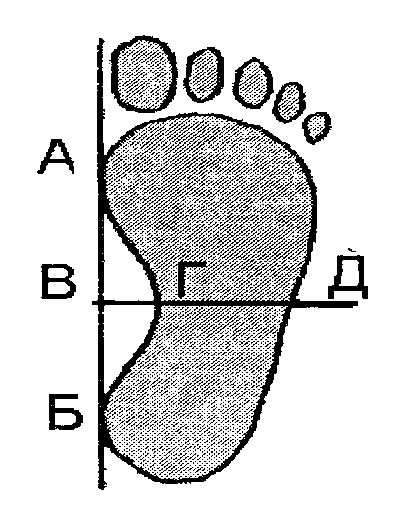
\includegraphics[width=0.4\textwidth]{striter.png} 
    \caption{Графическая схема разметки плантограммы для расчета индекса В.~А. Штритера.}
    \label{fig:sztriter}
\end{figure}

Данные стандартные медицинские методики расчета характеристик стопы основаны на
том, что врач-ортопед может визуально выделить контуры стопы на плантограмме,
определить необходимые контрольные точки и произвести расчет с использованием
линейки и ручки (для получения точных значений) и просто «на глаз», если не требуется
высокой точности.


\subsection{Поэтапное описание алгоритма анализа плантограммы}

Рассмотрим методику анализа состояния стопы на примере обработки фотоснимка подошвенной поверхности, полученного с помощью плантоскопа. Алгоритм состоит из десяти последовательных шагов, каждый из которых визуализирован на соответствующем рисунке.

\textbf{Шаг 1. Разделение на левую и правую стопы.} На вход алгоритма подается фотоснимок, полученный с помощью плантоскопа, на котором запечатлены обе стопы пациента, ориентированные носочной частью вниз. С помощью библиотеки \texttt{rembg} выполняется автоматическое удаление фона, после чего из альфа-канала выделяются два наибольших контура, соответствующих левой и правой стопе. Для каждого контура вычисляется ограничивающий прямоугольник (bounding box), и по координатам определяется линия разделения, проходящая посередине между стопами. Исходное изображение разделяется на две половины по данной линии. На отладочном изображении зеленой линией отображается граница разделения, синими контурами - выделенные стопы, красными прямоугольниками - их bounding boxes. Данная предобработка обеспечивает независимый анализ каждой стопы в единой системе координат.

\begin{figure}[H]
    \centering
    \includegraphics[width=0.40\textwidth]{../src/screenshots/split-feet.png}
    \caption{Шаг 1. Разделение на левую и правую стопы}
    \label{fig:step1}
\end{figure}

\textbf{Шаг 2. Исходное изображение стопы.} Полученная на предыдущем шаге половина снимка, содержащая отдельную стопу, поворачивается на 180° таким образом, чтобы носочная часть оказалась в верхней части кадра, а пятка - в нижней. Изображение правой стопы дополнительно отзеркаливается по горизонтали для унификации с левой стопой. Данная ориентация позволяет применять единую логику поиска анатомических точек и расчета индексов независимо от того, левая или правая стопа анализируется.

\begin{figure}[H]
    \centering
    \includegraphics[width=0.32\textwidth]{../src/screenshots/0-step-1-original.png}
    \caption{Шаг 2. Исходное изображение стопы после поворота и унификации}
    \label{fig:step2}
\end{figure}

\textbf{Шаг 3. Удаление фона.} С помощью библиотеки \texttt{rembg} выполняется автоматическое удаление фона вокруг стопы. На данном этапе формируется изображение с прозрачным фоном, где силуэт стопы отделен от подложки плантоскопа. Это позволяет исключить влияние элементов фона (бликов, артефактов стекла, краев кадра) на дальнейшие шаги обработки.

\begin{figure}[H]
    \centering
    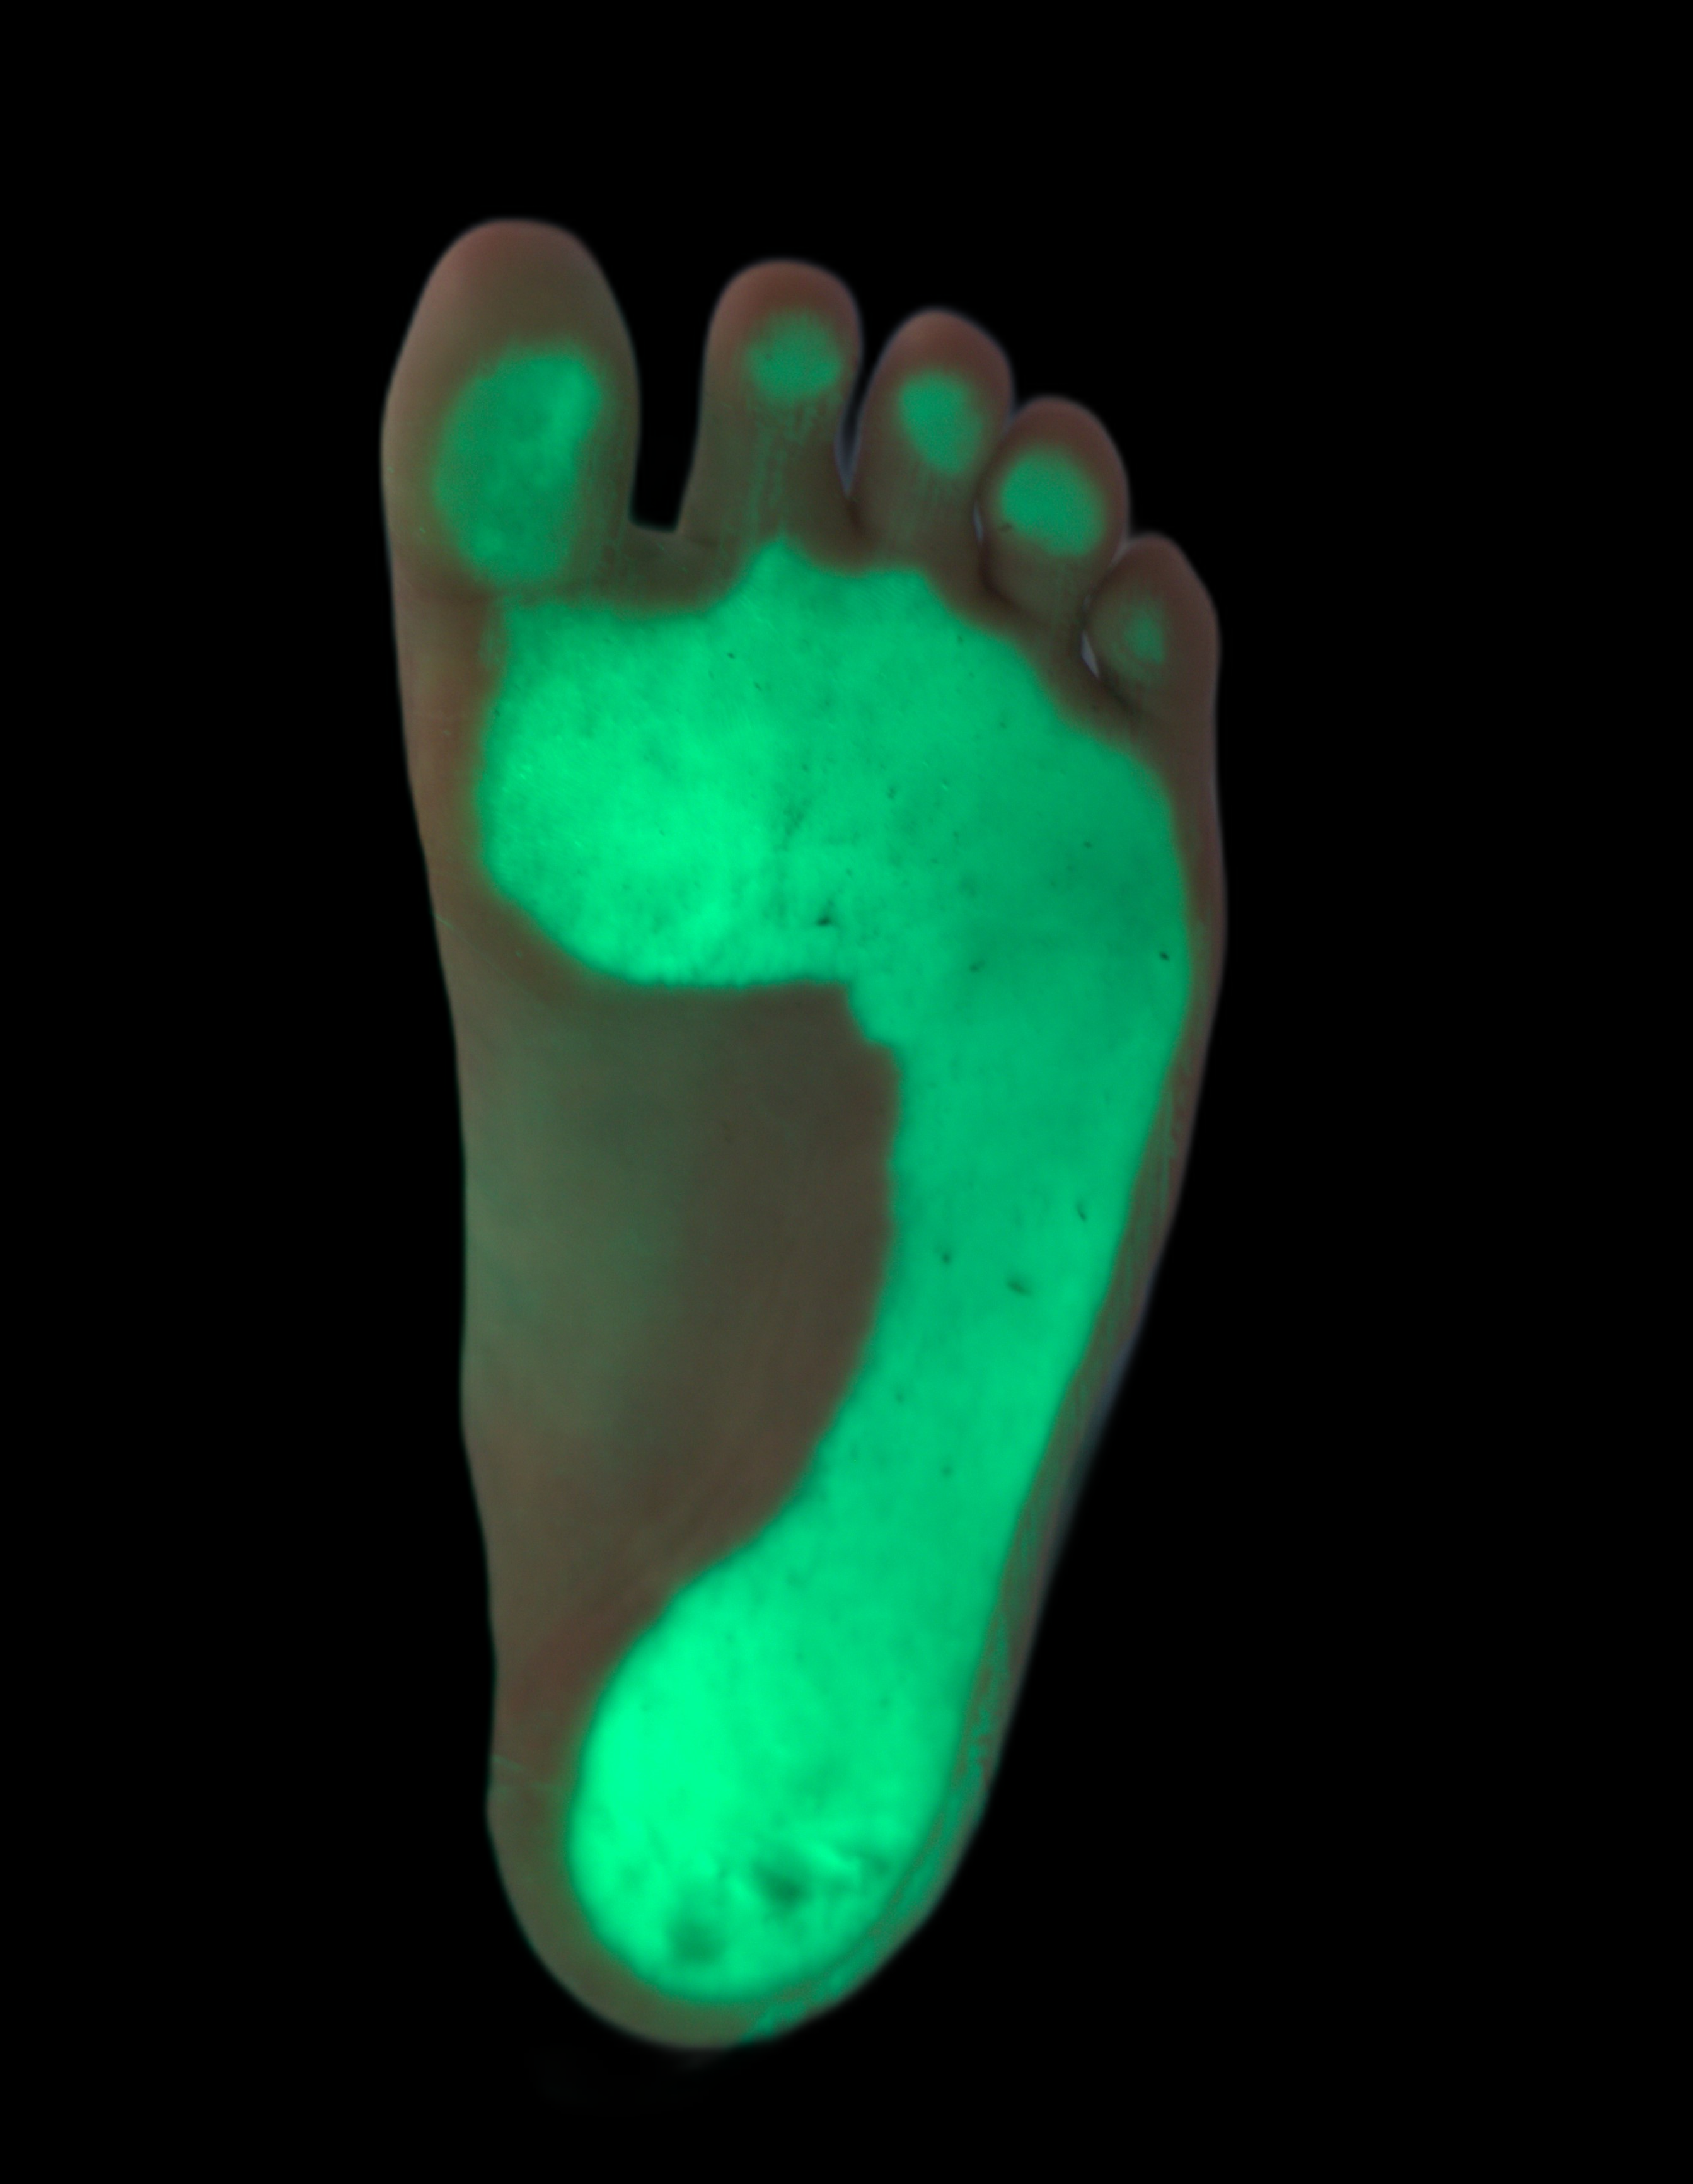
\includegraphics[width=0.32\textwidth]{../src/screenshots/0-step-2-remove-background.png}
    \caption{Шаг 3. Результат удаления фона}
    \label{fig:step3}
\end{figure}

\textbf{Шаг 4. Бинарная маска стопы.} Из альфа-канала, полученного после удаления фона, путем порогового преобразования с порогом 100 формируется бинарная маска стопы. К маске применяется морфологическая операция закрытия (\texttt{MORPH\_CLOSE}) с квадратным структурным элементом размером $5\times5$ пикселей. Данная операция устраняет мелкие разрывы и шумы, возникшие на этапе выделения стопы, и обеспечивает целостность силуэта.

\begin{figure}[H]
    \centering
    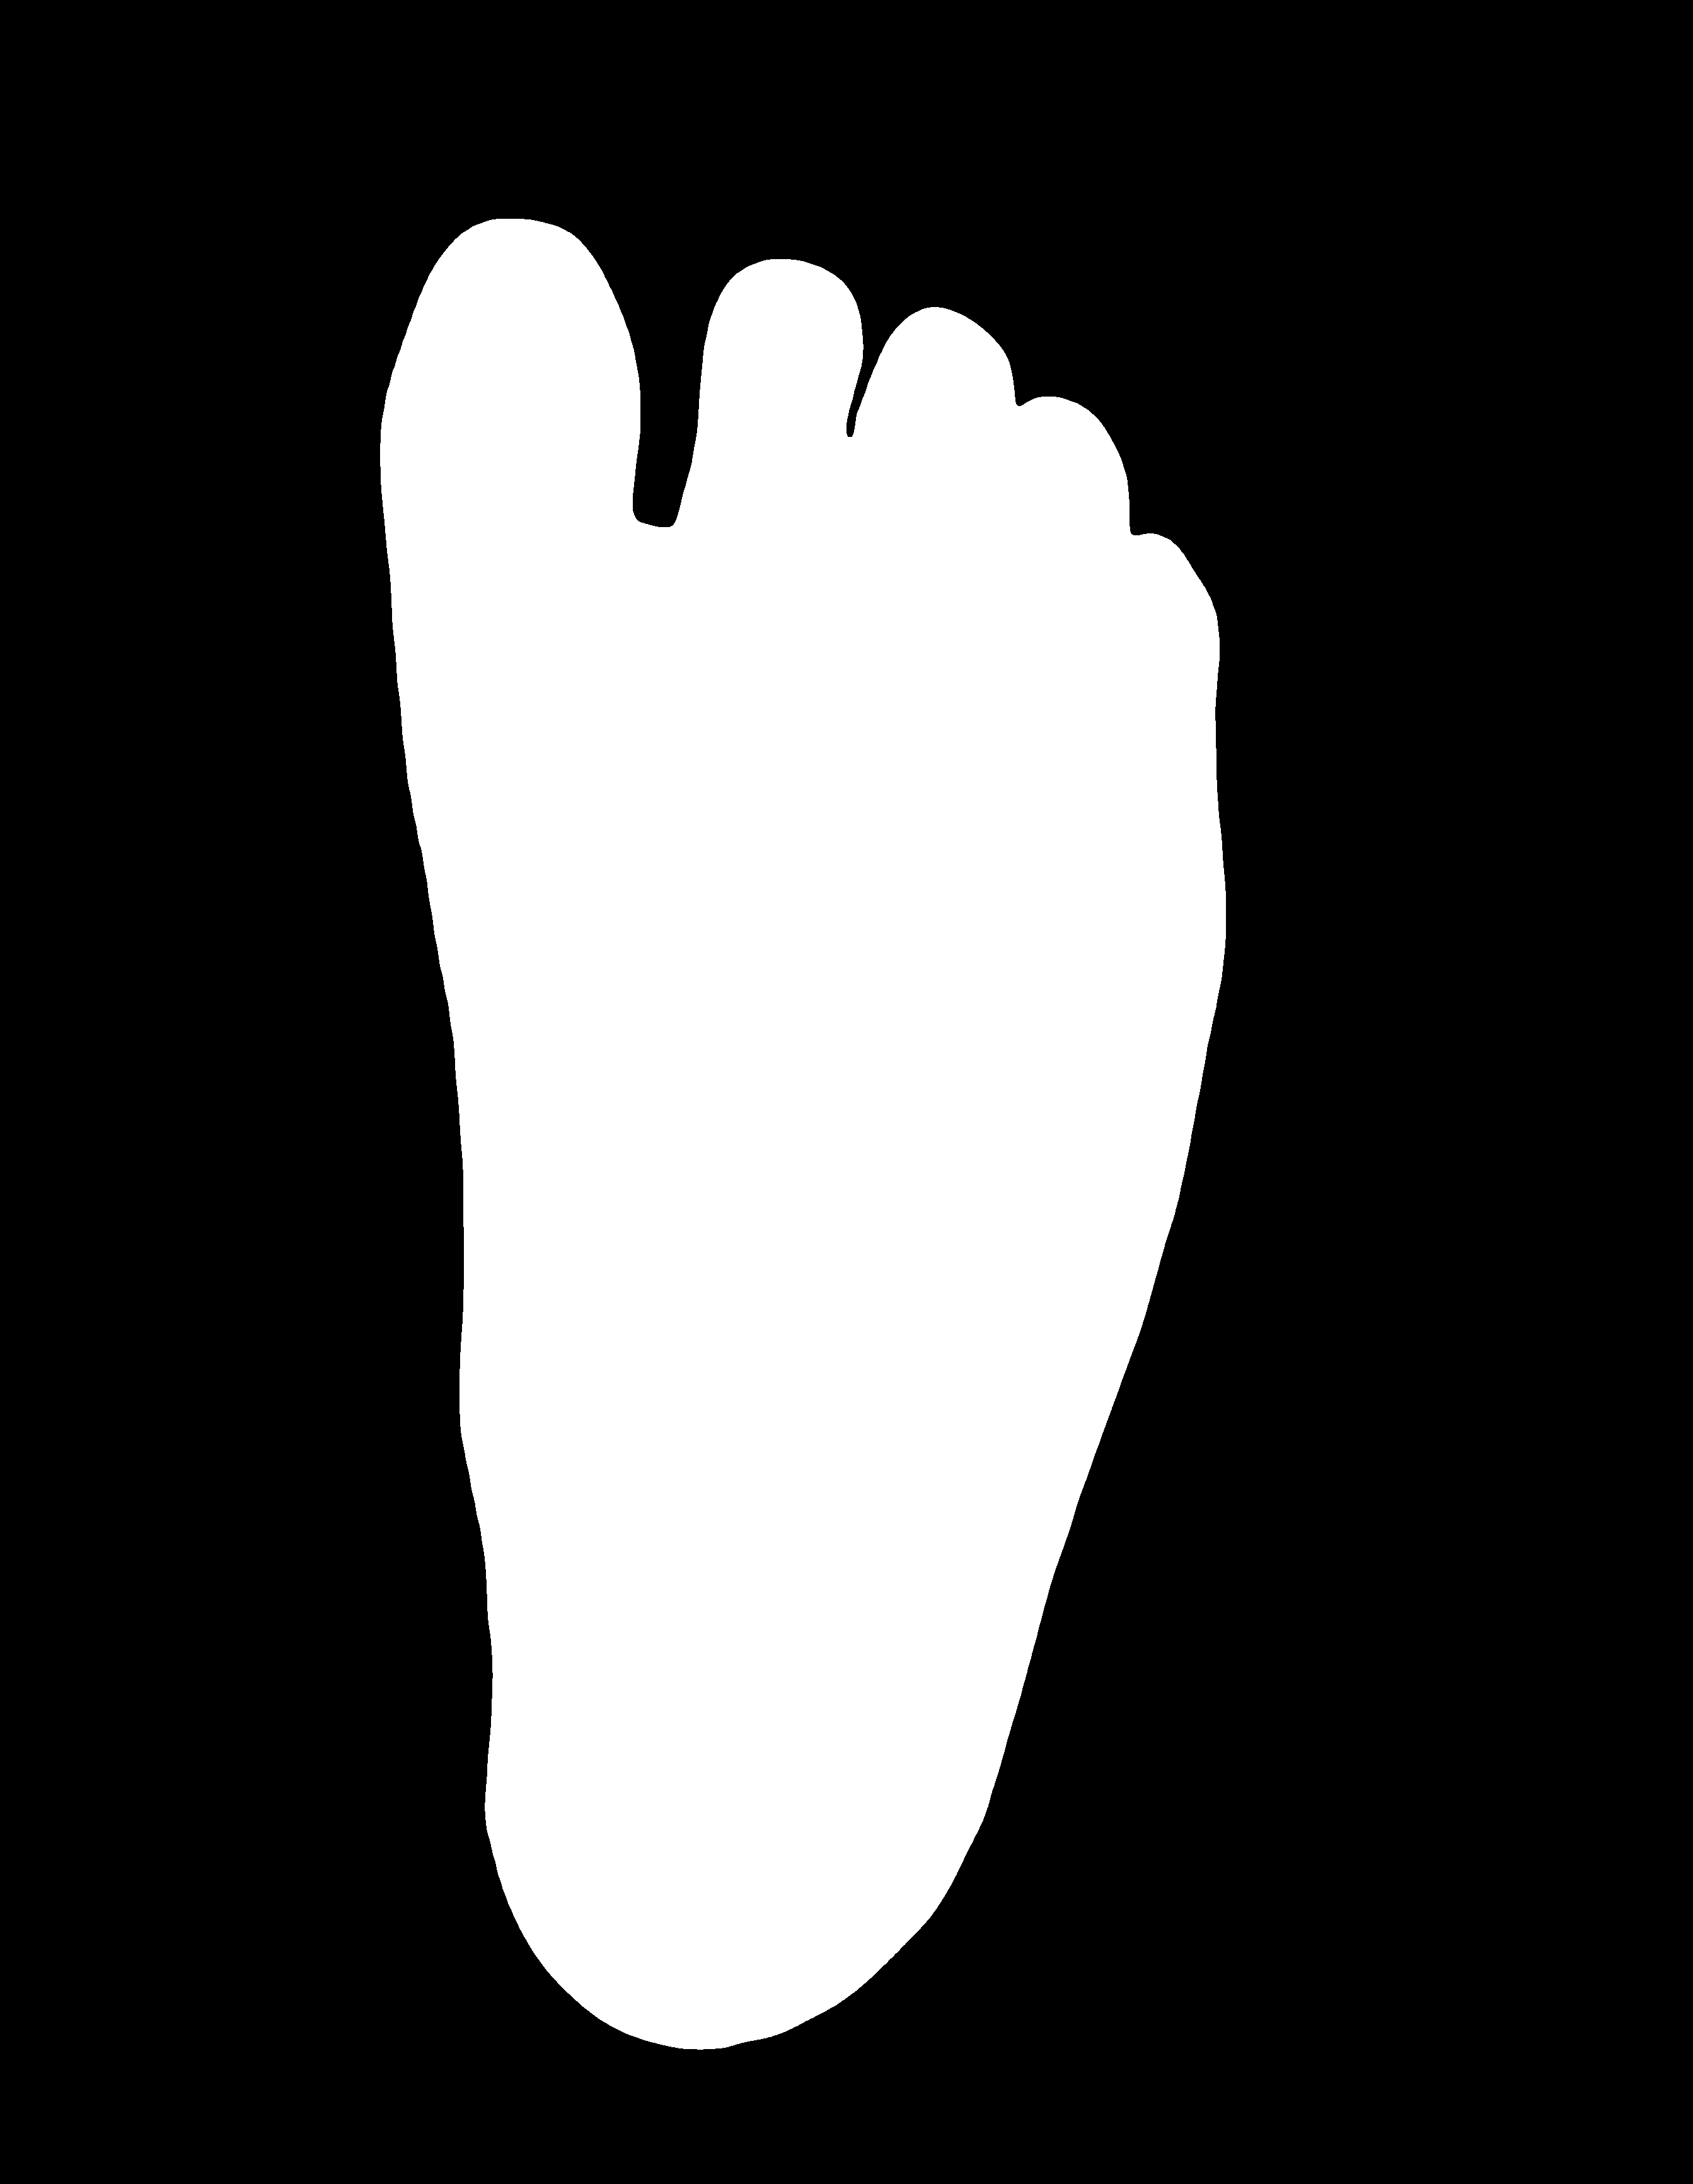
\includegraphics[width=0.32\textwidth]{../src/screenshots/0-step-3-foot-mask.png}
    \caption{Шаг 4. Бинарная маска стопы}
    \label{fig:step4}
\end{figure}

\textbf{Шаг 5. Контур стопы.} На исходном изображении стопы выполняется выделение внешнего контура. С помощью функции \texttt{cv2.findContours} в режиме \texttt{RETR\_EXTERNAL} находятся все внешние границы бинарной маски, после чего контур отрисовывается синим цветом. Полученный контур определяет границы стопы и используется в дальнейшем для ограничения области поиска плантограммы.

\begin{figure}[H]
    \centering
    \includegraphics[width=0.32\textwidth]{../src/screenshots/0-step-4-foot-contour.png}
    \caption{Шаг 5. Выделенный контур стопы}
    \label{fig:step5}
\end{figure}

\textbf{Шаг 6. Маска зеленого цвета.} Исходное изображение преобразуется из цветового пространства BGR в HSV. Затем с помощью функции \texttt{cv2.inRange} выделяются все пиксели, попадающие в заданный диапазон зеленого цвета: нижняя граница - $[74, 149, 141]$, верхняя - $[86, 255, 194]$. Данный диапазон соответствует цвету области контакта стопы с опорной поверхностью плантоскопа. Результатом является бинарная маска, в которой белым отмечены все пиксели зеленого цвета на изображении.

\begin{figure}[H]
    \centering
    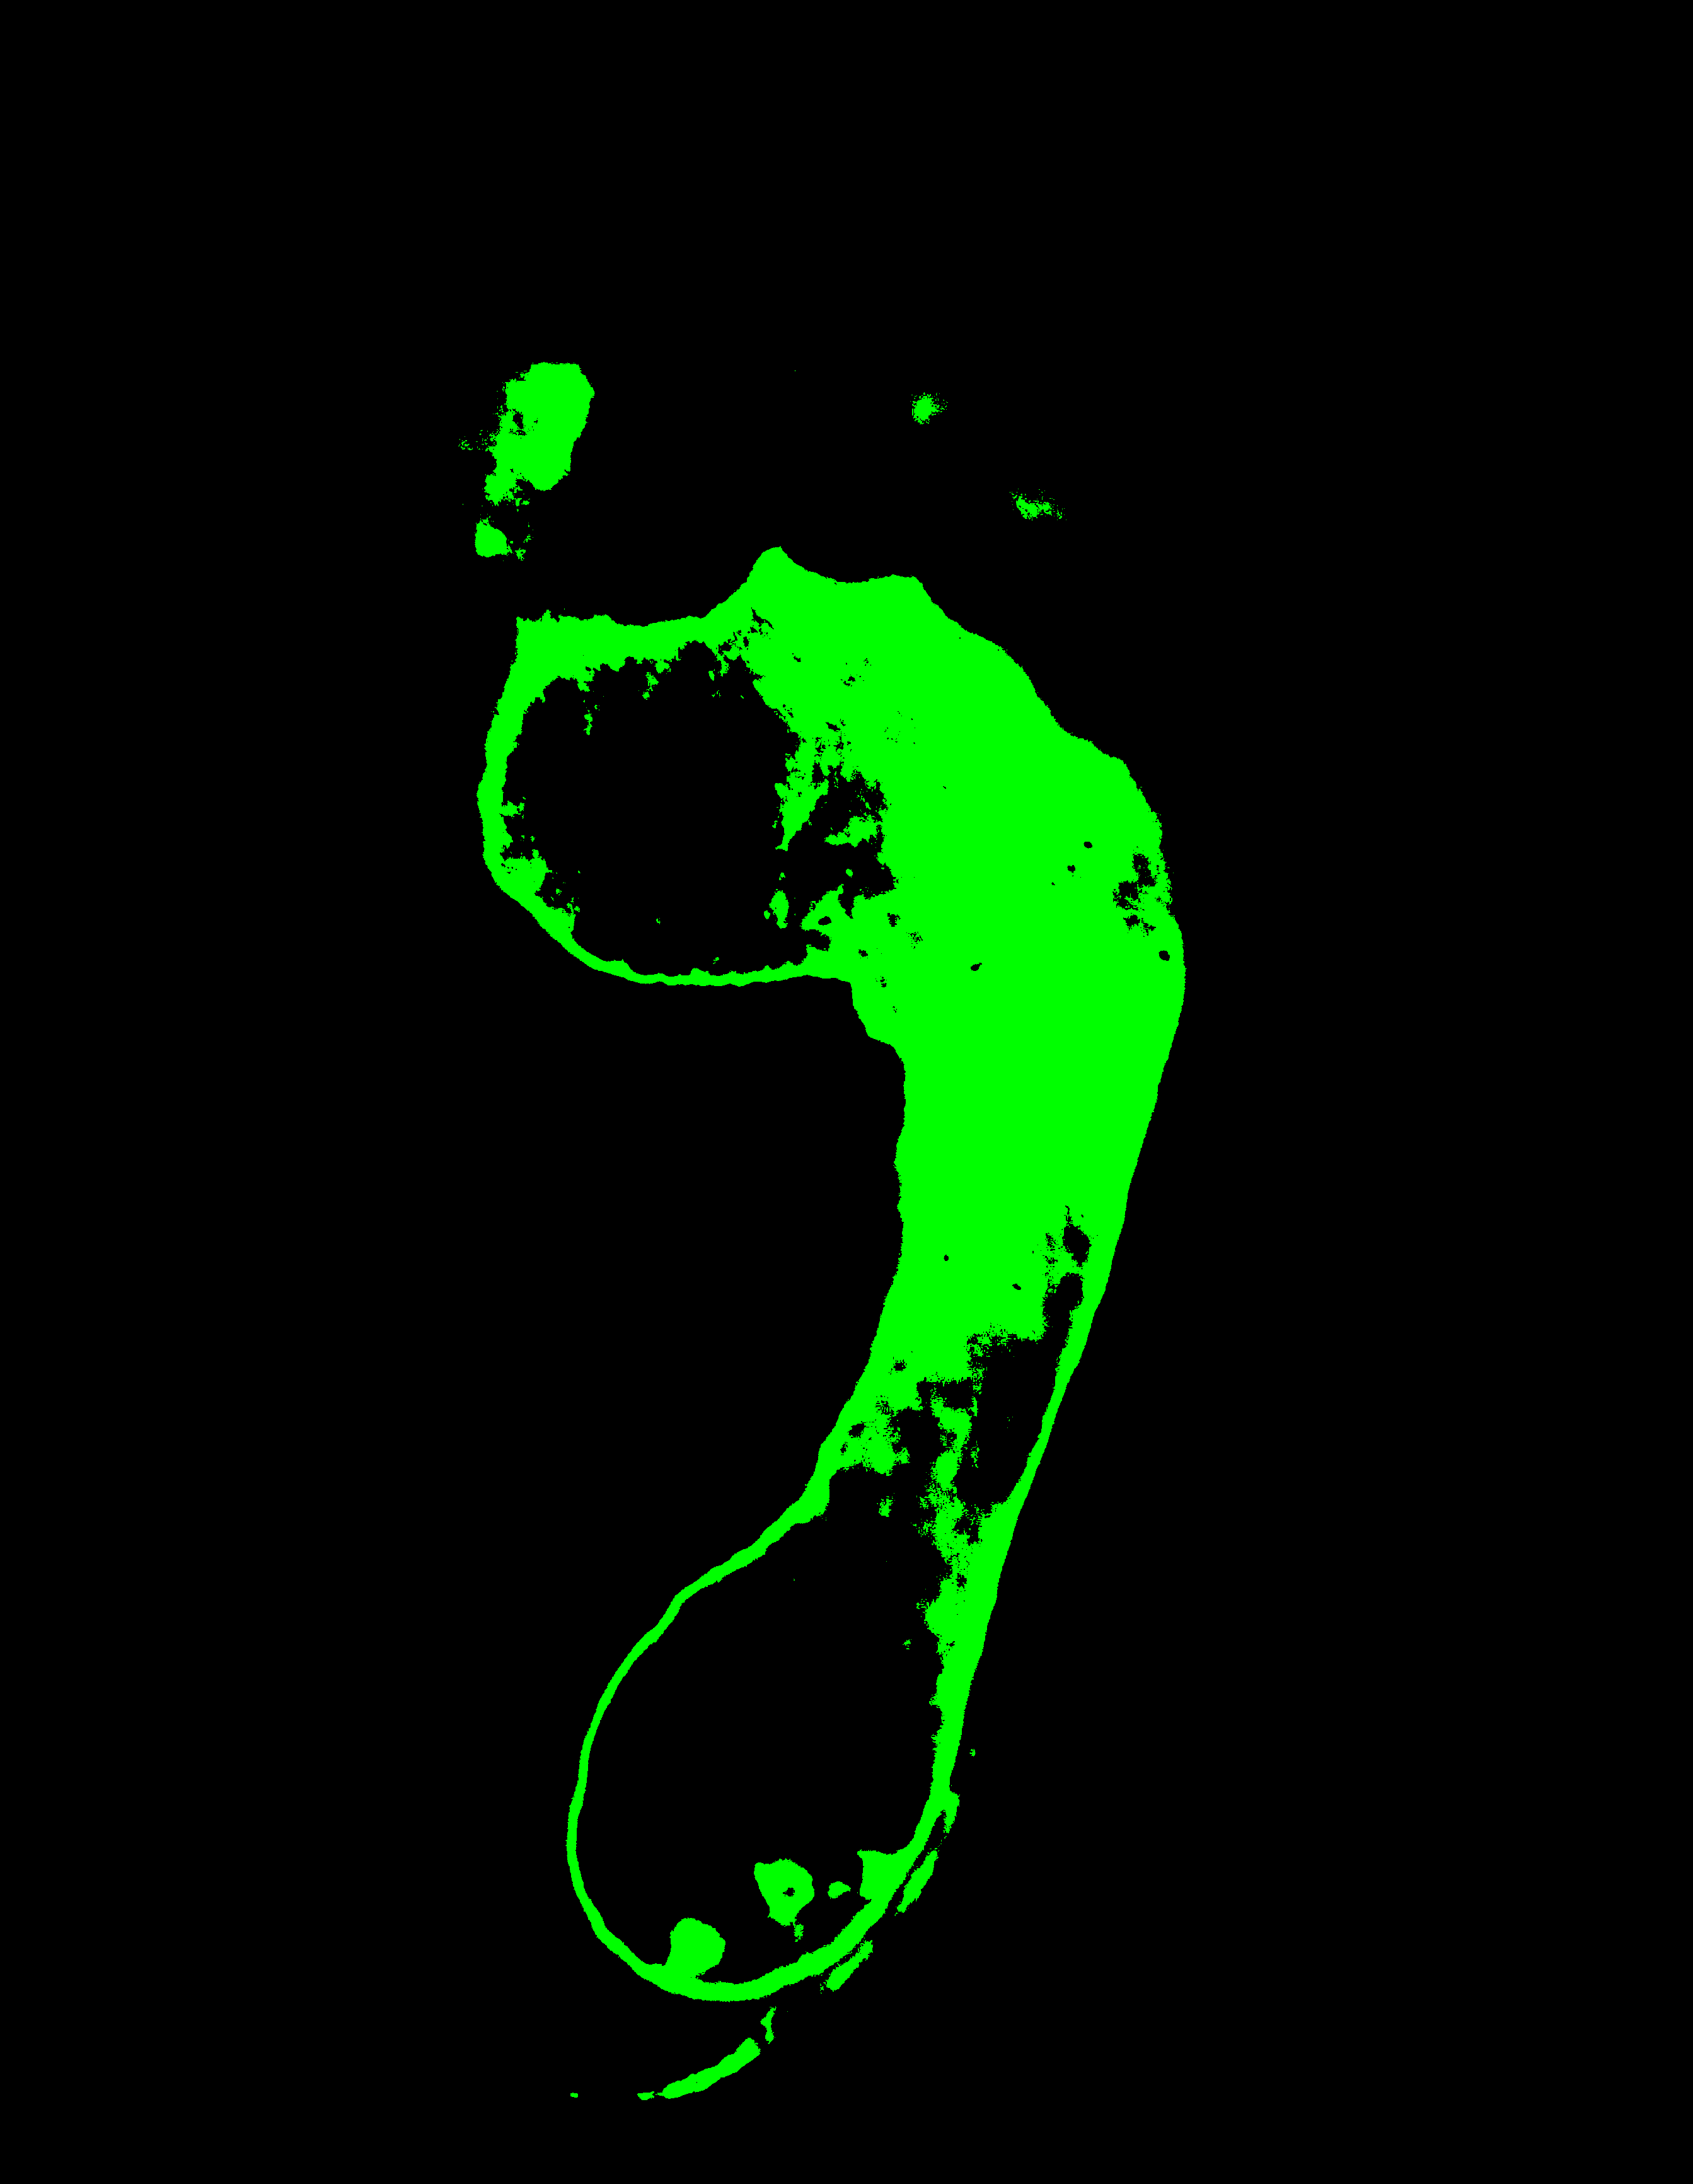
\includegraphics[width=0.32\textwidth]{../src/screenshots/0-step-5-green-mask-raw.png}
    \caption{Шаг 6. Маска зеленого цвета}
    \label{fig:step6}
\end{figure}

\textbf{Шаг 7. Фильтрация по площади.} Полученная на предыдущем этапе маска зеленого цвета логически умножается на маску стопы (операция \texttt{bitwise\_and}), что позволяет оставить только те зеленые области, которые находятся внутри контура стопы. После этого все связные области, площадь которых меньше 50\,000 пикселей, отбрасываются как шумовые. В результате формируется очищенная маска плантограммы, содержащая только значимую область контакта стопы с опорой.

\begin{figure}[H]
    \centering
    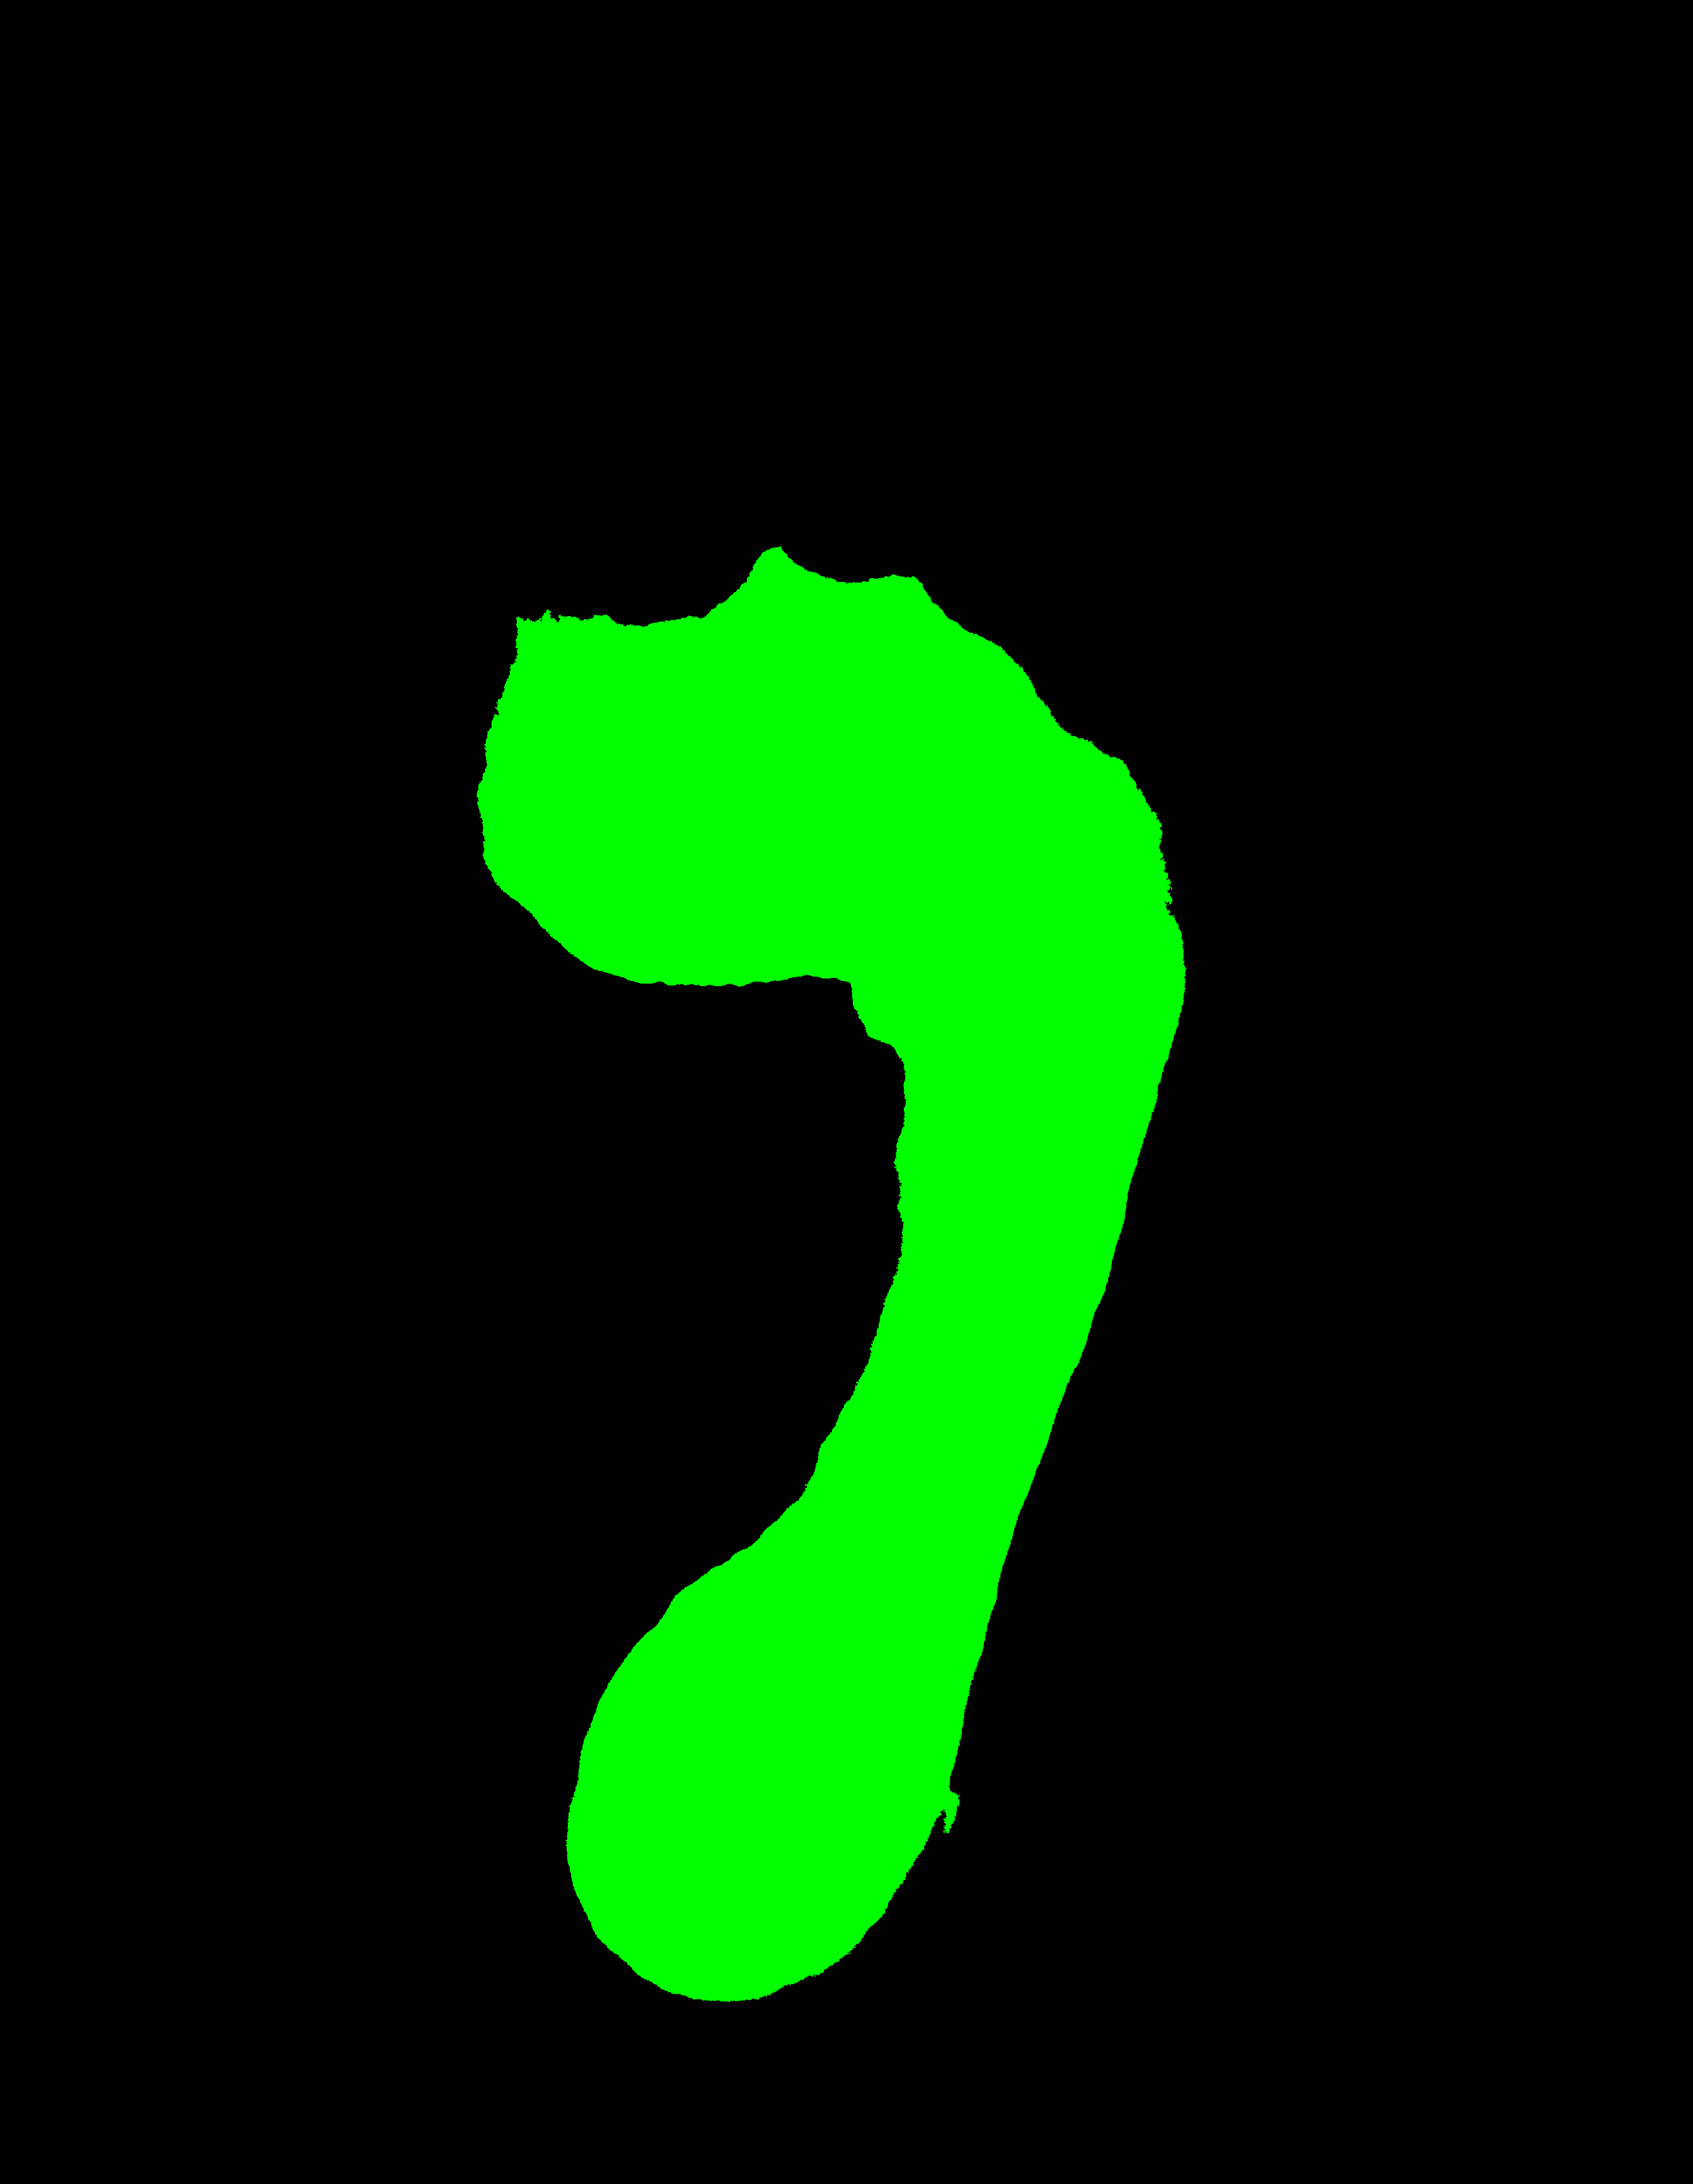
\includegraphics[width=0.32\textwidth]{../src/screenshots/0-step-6-plantogram-clean.png}
    \caption{Шаг 7. Очищенная маска плантограммы после фильтрации по площади}
    \label{fig:step7}
\end{figure}

\textbf{Шаг 8. Итоговое наложение контуров.} На исходное изображение стопы одновременно наносятся два контура: синий - контур стопы, полученный на шаге 5, и красный - контур плантограммы, полученный из очищенной маски шага 7. Данное изображение является итоговым результатом этапа предобработки и служит основой для последующего вычисления анатомических индексов.

\begin{figure}[H]
    \centering
    \includegraphics[width=0.32\textwidth]{../src/screenshots/0-step-7-all-contours.png}
    \caption{Шаг 8. Итоговое наложение контуров стопы и плантограммы}
    \label{fig:step8}
\end{figure}

\textbf{Шаг 9. Точки A и B, линия AB.} На итоговом изображении выполняется поиск двух ключевых анатомических точек. Точка $A$ определяется как крайняя левая точка в самой широкой части носочной области плантограммы (верхние 30\% высоты контура). Точка $B$ находится как крайняя левая точка в области пятки (нижние 35\% высоты контура). На изображение наносятся обе точки с буквенными обозначениями и соединяющая их линия $AB$ желтого цвета. Данные точки являются базовыми для расчета индекса Штриттера.

\begin{figure}[H]
    \centering
    \includegraphics[width=0.32\textwidth]{../src/screenshots/0-step-8-points-AB.png}
    \caption{Шаг 9. Точки $A$ и $B$ с линией $AB$}
    \label{fig:step9}
\end{figure}

\textbf{Шаг 10. Индекс Штриттера.} Через середину отрезка $AB$ (точка $V$) строится перпендикуляр к линии $AB$ фиолетового цвета. Определяются точки пересечения данного перпендикуляра с контуром плантограммы: точка $G$ (внутренний край, желтая) и точка $D$ (наружный край, голубая). Индекс Штриттера вычисляется по формуле:

\begin{equation}
    I = \frac{GD}{VD} \times 100\%,
\end{equation}

\noindent где $GD$ - длина отрезка между внутренним и наружным краем плантограммы по перпендикуляру, $VD$ - расстояние от центра отрезка $AB$ до наружного края. На изображение наносятся все пять точек ($A$, $B$, $V$, $G$, $D$) с буквенными обозначениями, линия $AB$, перпендикуляр и крестик в точке $V$. По полученному значению индекса определяется тип стопы: высокосводчатая (полая) - до 36, повышенный свод - 36--43, нормальная - 43--50, уплощенная - 50--60, плоскостопие - свыше 60.

\begin{figure}[H]
    \centering
    \includegraphics[width=0.32\textwidth]{../src/screenshots/0-step-9-strieter-index.png}
    \caption{Шаг 10. Результат расчета индекса Штриттера с построением всех точек}
    \label{fig:step10}
\end{figure}

\subsection{Алгоритм анализа плантограммы с использованием генетического
алгоритма}
\subsubsection{Подготовка данных}
\subsubsection{Генетический алгоритм для подбора параметров алгоритма
оконтуривания плантограммы}
\subsubsection{Алгоритм расчета контрольных линий и точек плантограммы}
\subsection{Алгоритм анализа плантограммы с использованием нейронных
сетей
}
\subsubsection{Архитектура сети}
\subsubsection{Обучение сети}
\subsection{Обработка полученных результатов с помощью алгоритмов
компьютерного зрения}


\conclusion
Актуальность разработки и внедрения цифровых медицинских технологий в настоящее
время признается в рамках междисциплинарного консенсуса специалистов.
% Отобразить все источники. Даже те, на которые нет ссылок.
% \nocite{*}


Диагностика деформаций стопы является актуальной проблемой, такие заболевания характеризуются высокой частотой встечаемости среди людей всех возрастных групп. Плантография получила широкое распространение в клинической практике среди объективных количественных методов диагностики плоскостопия, она основана на оценке отпечатков подошвенной поверхности стопы. Оценка и анализ эффективности методов автоматической оценки с помощью "компьютерного зрения" являются основной целью исследования.В
исследовании рассматриваются методы автоматического распознавания и разметки фотоплантограмм
стопы с использованием генетических алгоритмов и нейронных сетей для построения контрольных
точек стопы на примере вычисления индексов продольного и поперечного сводов стопы.

\bibliographystyle{ugost2003}
\bibliography{thesis}

% Окончание основного документа и начало приложений Каждая последующая секция
% документа будет являться приложением
\appendix


\section{Приложение}
\section{Коды}



Функция \texttt{resize\_with\_padding} приводит изображение к фиксированному
размеру $512\times512$ пикселей, сохраняя пропорции и добавляя чёрные полосы.
Коэффициент масштабирования $\mathrm{scale} = \min(t_w / w,\; t_h / h)$
выбирается по меньшей стороне, чтобы исключить обрезание. Новые размеры
$\mathrm{new\_w}, \mathrm{new\_h}$ вычисляются умножением исходных на
$\mathrm{scale}$ с округлением до целого, после чего вызывается \texttt{cv2.resize}
с интерполяцией \texttt{INTER\_AREA}, оптимальной для уменьшения. Чёрный холст
нужного размера заполняется масштабированным изображением по центру. Смещения
$\mathrm{dx}$ и $\mathrm{dy}$ рассчитываются как половина разности между
целевыми и новыми размерами. Функция возвращает изображение со строго
заданными габаритами и неискажёнными пропорциями исходного объекта.

\begin{Verbatim}[
  numbers=left,
  breaklines=true,
  breakanywhere=true
]

\end{Verbatim}

Функция \texttt{split\_feet\_smart} разделяет изображение с двумя стопами по промежутку
между ними и применяет нормализующие преобразования. Сначала вызывается
\texttt{remove} для удаления фона, и из альфа-канала $mask$ бинаризацией
получается чёрно-белая маска. Функция \texttt{cv2.findContours} выделяет
внешние контуры и оставляет два крупнейших по площади --- это левая и правая
стопы. Для каждого контура вычисляется ограничивающий прямоугольник
\texttt{boundingRect}; прямоугольники сортируются по координате $x$. Линия
разреза $\mathrm{split\_x}$ проходит посередине между правым краем левого
прямоугольника и левым краем правого. Левая стопа вырезается как
\texttt{src\_image[:, :split\_x]} и поворачивается на $180^\circ$, правая ---
как \texttt{src\_image[:, split\_x:]} с поворотом на $180^\circ$ и
горизонтальным отражением \texttt{cv2.flip}. В режиме отладки на копии
изображения отрисовываются линия разреза, ограничивающие прямоугольники и
контуры. Функция возвращает кортеж из двух или трёх изображений.


\end{document}